\documentclass[letterpaper,12pt]{article}
\usepackage[top = 1in, bottom = 1in, left = 0.5in, right = 1in]{geometry}
\usepackage{inputenc}
\usepackage{graphicx}
\usepackage{amsmath}
\usepackage{amsfonts}
\usepackage{caption}
\usepackage{color}
\usepackage{listings}
\usepackage[framed,numbered,autolinebreaks,useliterate]{mcode}
%opening
\author{Gowtham Garimella}

\makeatletter
\newcommand\ackname{Acknowledgements}
\if@titlepage
  \newenvironment{acknowledgements}{%
      \titlepage
      \null\vfil
      \@beginparpenalty\@lowpenalty
      \begin{center}%
        \bfseries \ackname
        \@endparpenalty\@M
      \end{center}}%
     {\par\vfil\null\endtitlepage}
\else
  \newenvironment{acknowledgements}{%
      \if@twocolumn
        \section*{\abstractname}%
      \else
        \small
        \begin{center}%
          {\bfseries \ackname\vspace{-.5em}\vspace{\z@}}%
        \end{center}%
        \quotation
      \fi}
      {\if@twocolumn\else\endquotation\fi}
\fi
\makeatother

\newcommand{\executeiffilenewer}[3]{%
\ifnum\pdfstrcmp{\pdffilemoddate{#1}}%
{\pdffilemoddate{#2}}>0%
{\immediate\write18{#3}}\fi%
}
\newcommand{\includesvg}[1]{%
\executeiffilenewer{#1.svg}{#1.pdf}%
{inkscape -z -D --file=#1.svg %
--export-pdf=#1.pdf --export-latex}%
\input{#1.pdf_tex}%
}

\title{EN.530.603 Applied Optimal Control \\HW \#1 Solutions}
\graphicspath{{./figures/}}
\begin{document}
\maketitle

\begin{enumerate}

  %%%%%%%%%%%%%%%Question 1%%%%%%%%%%%%%%%%%%%%%%%%
\item To find stationary points and determine whether they are maxima, minima or
saddle points:
  For stationary points, the gradient has to be zero.
  \begin{enumerate}
   \item  %%%%%%Part A%%%%%%%%%%%
   \begin{align*}
      L(x) &= (1-x_1)^2 + 100(x_2 - x_1^2)^2 \\[6pt]
      \nabla L(x) = \begin{bmatrix}
			  \frac{\partial L}{\partial x_1} \\[6pt]
			  \frac{\partial L}{\partial x_2} \\
			  \end{bmatrix}  &= 
			  \begin{bmatrix}
			    2(1-x_1)(-1) + 200(x_2 - x_1^2)(-2x_1) \\
			    2\times 100 (x_2 -x_1^2)\\
			    \end{bmatrix}  = \mathbf{0_{2\times1}}\\[6pt]
	\Rightarrow x_2 = x_1^2 \quad &	\& \quad -1+x_1 = 0\\
	\Rightarrow x_1 = 1 \quad & \& \quad x_2 = x_1^2 = 1 \\
   \end{align*}
   Thus the stationary point is (1,1). Now to characterize the stationary point
we look at the Hessian of the function:
   \begin{align*}
    \nabla^2 L(x) &= \begin{bmatrix}
                     2\left( 1 - 200 x_2 + 600 x_1^2\right) & 2 (-200 x_1) \\
                     200(-2 x_1) & 200 \\
                    \end{bmatrix}\\[6pt]
     \nabla^2 L(x) |_{(1,1)} &= H =  \begin{bmatrix}
                                802 & -400 \\
                                -400 & 200 \\
                               \end{bmatrix}\\
      eig(H) &= \{1001.6, 0.4\}\\
   \end{align*}
   Thus the Hessian is positive definite which implies the stationary point
(1,1) is a \textbf{strict local minima}
   
   \item %%%%%%Part B%%%%%%%%%%%
   \begin{align*}
    L(u) &= (u-1)(u+2)(u-5) \\
    \nabla L(u) = \frac{\partial L}{\partial u} &= (u-1)(u+2) + (u-1)(u-5) +
(u+2)(u-5) = 3 u^2 -8u -7 = 0\\
    \Rightarrow u^* &= \{3.36, -0.69\}\\
  \end{align*}
  Now to characterize the stationary points we look at the Hessian:
  \begin{align*}
   \nabla^2 L(u) = \frac{\partial^2 L}{\partial^2 u} &= 6u -8\\
   \nabla^2 L(u) |_{u = 3.36} &= 6 (3.36) - 8 = 12.16 \\
   \nabla^2 L(u) |_{u = -0.694} &= 6 (-0.694) - 8 = -12.16 \\
  \end{align*}
  Clearly, point u = 3.36 is \textbf{strict local minima} and point u = -0.694
is \textbf{strict local maxima}
  
  \item %%%%%%Part C%%%%%%%%%%%
  \begin{align*}
    L(u) &= (u_1^2 + 3 u_1 - 4) (u_2 ^2 - u_2 + 6) \\
    \nabla L(u) = \begin{bmatrix}
			  \frac{\partial L}{\partial u_1} \\[6pt]
			  \frac{\partial L}{\partial u_2} \\
			  \end{bmatrix}  &= 
			  \begin{bmatrix}
			    (2 u_1 + 3) (u_2^2 -u_2 + 6) \\
			    (u_1^2 + 3u_1 -4) (2 u_2 -1) \\
			    \end{bmatrix}  = \mathbf{0_{2\times1}}\\[6pt]
	\forall u_2 &\in \mathbb{R} \quad u_2^2 - u_2 + 6 > 0 \\	 
	\Rightarrow u_1 &= -3/2 \\
	\Rightarrow u^* &= \begin{bmatrix}
	                 -3/2 \\
	                 1/2 \\
	                \end{bmatrix}\\
  \end{align*}
  Now that we found the stationary point let us characterize it by looking at
the Hessian of the above objective function:
  \begin{align*}
   \nabla^2 L(u) &= \begin{bmatrix}
                    2 (u_2^2 -u_2 + 6) & (2u_1+3)(2u_2-1) \\
                    (2u_1+3)(2u_2 - 1) & 2(u_1^2 +3 u_1 - 4) \\
                   \end{bmatrix} \\
    \nabla^2 L(u) |_{u = (-1.5,0.5)} &= \begin{bmatrix}
                                         11.5 & 0 \\
                                         0 & -12.5\\
                                        \end{bmatrix}\\
     \Rightarrow eig(\nabla^2 L(u)) &= \{ 11.5,-12.5\} \\
  \end{align*}
  Since the eigen values are both positive and negative at the stationary point
u = (-3/2, 1/2), the point is a \textbf{saddle point}. 
  \end{enumerate}
  
  
  %%%%%%%%%%%%%%%Question 2%%%%%%%%%%%%%%%%%%%%%%%%
  \item To find the stationary points and determine the maxima, minima or saddle
points:
  \begin{enumerate}
   \item %%%%%%Part A%%%%%%%
   Define $L^\prime$  using lagrangian multipliers as $L^\prime := L(x) +
\lambda f(x)$ where $\lambda \in \mathbb{R}$ is a scalar. To find the stationary
points, we have to equate the gradient to zero:
   \begin{align*}
    L^\prime (x) &= \frac{1}{2} (x_1^2 + x_2^2 + x_3^2) + \lambda (x_1 + x_2 +
x_3) \\
    \frac{\partial L^\prime}{\partial x_1} &= x_1 + \lambda  = 0  \quad
\text{(at stationary point)}\\
    \Rightarrow \lambda &= -x_1^* \quad (x_1^* \text{ is the stationary
point})\\
    \frac{\partial L^\prime}{\partial x_2} &= x_2 + \lambda  = 0  \\
    \frac{\partial L^\prime}{\partial x_3} &= x_3 + \lambda  = 0  \\
    \text{From constraint  f(x) }\quad  &x_1 + x_2 + x_3 = 0 \\
    \Rightarrow x_2^* = x_3^* &= x_1^* = \lambda = 0\\
   \end{align*}
   Thus the stationary point is (0,0,0). To characterize the stationary point we
look at the Hessian of the $L^\prime$. Since $\lambda = 0$, $L^\prime = L$.
Thus 
   \begin{align*}
    \nabla^2 L^\prime = \nabla^2 L = H = \begin{bmatrix}
                                      1 & 0 & 0 \\
                                      0 & 1 & 0 \\
                                      0 & 0 & 1 \\
                                     \end{bmatrix}
    \Rightarrow eig(H) = \{1,1,1\}                                     
   \end{align*}
   Since the eigen values are all positive, the Hessian is positive definite and
hence the stationary point (0,0,0) is a \textbf{strict local minima}
   
   \item %%%%%%Part B%%%%%%%
    As in above equation define the augmented cost function and let's equate the
gradient to zero:
    \begin{align*}
     &L^\prime(u) = L(u) + \lambda f(u) = (u_1^2 + 3 u_1 - 4) (u_2^2 - u_2 + 6)
+ \lambda (u_1 - 2 u_2) \\
     &\frac{\partial L^\prime}{\partial u_1} = (2 u_1 + 3)(u_2^2 - u_2 + 6) +
\lambda = 0 \quad \text{(at stationary point)} \\
     &\frac{\partial L^\prime}{\partial u_2} = (u_1^2 + 3 u_1 - 4)(2 u_2 - 1) -
2 \lambda = 0 \quad \text{(at stationary point)} \\
     &\frac{\partial L^\prime}{\partial \lambda} = u_1 - 2u_2 = 0 \\
     &\Rightarrow u_1 = 2u_2 \quad \text{and}\\
     &\Rightarrow (u_1^2 + 3 u_1 - 4)(2 u_2 - 1) + 2 (2 u_1 + 3)(u_2^2 - u_2 +
6) = 0\\
     &\Rightarrow (2 u_2^2 + 3 u_2 -2)(2 u_2 -1) +  (4 u_2 + 3)(u_2^2 - u_2 + 6)
= 0\\
     &\Rightarrow 8 u_2^3 + 3 u_2^2 +14 u_2 + 20 = 0
    \end{align*}
    The above cubic equation yields only one real root i.e $u_2 = -1.03$ i.e $u
= (-0.515,-1.03)$. To characterize this stationary point we look at the Hessian
of $L^\prime$:
    \begin{align*}
     \nabla^2 L^\prime &= \begin{bmatrix}
			    2(u_2^2 - u_2 + 6) & (2u_1 + 3) (2 u_2 - 1) \\
			    (2 u_1 + 3) (2 u_2 -1) & 2(u_1^2 + 3 u_1 - 4) \\
                         \end{bmatrix}\\
     \nabla^2 L^\prime |_{u=(-0.515,-1.03)} = H &= \begin{bmatrix}
                                              16.182 & -6.028 \\
                                              -6.028 & -10.56 \\
                                             \end{bmatrix} \quad \\
     eig(H) &= \{17.48,-11.86\}                                            
    \end{align*}
    Since the eigen values of the Hessian are positive and negative, the
stationary point(-0.515,-1.03) is a \textbf{saddle point}.
  \end{enumerate}
  
  %%%%%%%%%%%%%%%Question 3%%%%%%%%%%%%%%%%%%%%%%%%
  \item To optimize the quadratic cost function with constraints given as:
  \begin{align*}
    L(x,u) &= \frac{1}{2} x^T Q x + \frac{1}{2} u^T R u \\
    f(x,u) &= Ax + Bu + c = 0 \quad x \in \mathbb{R}^n, c \in \mathbb{R}^m\\
  \end{align*}
  Using the Lagrangian multipliers method:
  \begin{align*}
   L^\prime(x,u) &= \frac{1}{2} x^T  Q x + \frac{1}{2} u^T  R u + \lambda^T
(Ax+Bu+c)\\
   \frac{\partial L^\prime}{\partial x} &= x^T  Q  + \lambda^T (A) =
\mathbf{0_{1\times n}}\\
   \frac{\partial L^\prime}{\partial u} &= u^T  R  + \lambda^T (B) =
\mathbf{0_{1\times m}}\\
   \frac{\partial L^\prime}{\partial \lambda} &= Ax + Bu +c = 0 \\
  \end{align*}
  Since Q and R are both positive definite, they are invertible.
  \begin{align*}
   \Rightarrow x^T &= -\lambda^T A  Q^{-1} \\
   \Rightarrow u^T &=  -\lambda^T B  R^{-1}\\
   A x + B u = c  \quad &\equiv \left(A  {Q^T}^{-1} A^T + B {R^T} ^{-1} B^T
\right) \lambda = c\\
  \end{align*}
  For such a $\lambda$ to exist,
  \begin{equation*}
  c \in span\{A {Q^T}^{-1} A^T + B {R^T}^{-1} B^T \}
  \end{equation*}
 
  
  Second order sufficient condition requires:
  \begin{align*}
  dy^T \nabla^2 L^\prime dy = H = dy^T \begin{bmatrix}
                        Q & \mathbf{0_{n\times m}} \\
                       \mathbf{0_{m\times n}} &  R \\
                      \end{bmatrix} dy > 0\\
  \end{align*}
  Since  $Q$ and $R$ are both positive definite,
  \begin{equation*}
   \begin{bmatrix}
    x & u\\
   \end{bmatrix}
   \begin{bmatrix}
	Q & \mathbf{0_{n\times m}} \\
	\mathbf{0_{m\times n}} & R \\
   \end{bmatrix} 
   \begin{bmatrix}
    x^T \\
    u^T \\
   \end{bmatrix} = x^T  Q x + u^T R u > 0
  \end{equation*}
  Thus the Hessian is already positive definite and hence there is no required
second order sufficiency condition. Which implies that the necessary and
sufficient condition for minimizing the objective function is as given below:
  \begin{align*}
 \{ A  {Q^T}^{-1} A^T &+ B {R^T} ^{-1} B^T \} \lambda = c\\
  x &= -{Q^T}^{-1} A^T \lambda   \\
  u &= -{R^T}^{-1} B^T \lambda   \\
  \end{align*}

\item 
   Matlab code for both the parts are given as follows:
  \lstinputlisting[language=Matlab]{Hw1.m}
  \begin{enumerate}
    \item  The above solution converges to $\{x,u\} = \{1,1\}$ for very small
step sizes. If the step size is larger, the solution does not converge and even
diverges.
  \item The analytical solution for minimization following lagrangian method is
as follows:
  \begin{align*}
   L^\prime(x,u) &= x^2 + 10 u^2 + \lambda (x-2u+3) \\
   \frac{\partial L^\prime}{\partial x} &= 2x + \lambda = 0\\
   \frac{\partial L^\prime}{\partial u} &= 20u + 2\lambda = 0\\
   \frac{\partial L^\prime}{\partial \lambda} &= x-2u+3 = 0\\
   \Rightarrow \frac{-\lambda}{2} -&2\frac{\lambda}{10} + 3 = 0\quad \Rightarrow
\{\lambda,x,u\} = \{\frac{30}{7}, \frac{-15}{7}, \frac{-3}{7}\}\\
  \end{align*}
  The above solutions match with fmincon implementation from matlab.
  \end{enumerate}

  \begin{figure}[h!]
      \begin{minipage}{0.5\linewidth}
        \centering
	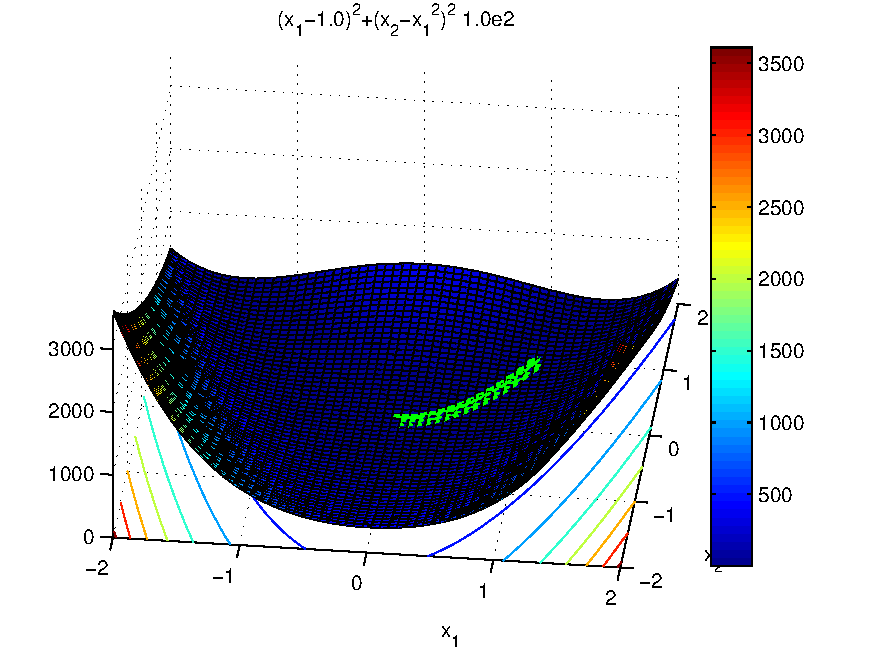
\includegraphics[width=4in, height = 3in]{pic1.pdf}
	\caption{(a) plot of L(x) and gradient descent}
      \end{minipage}
      \hspace{0.2in}
      \begin{minipage}{0.5\linewidth}
      \centering
	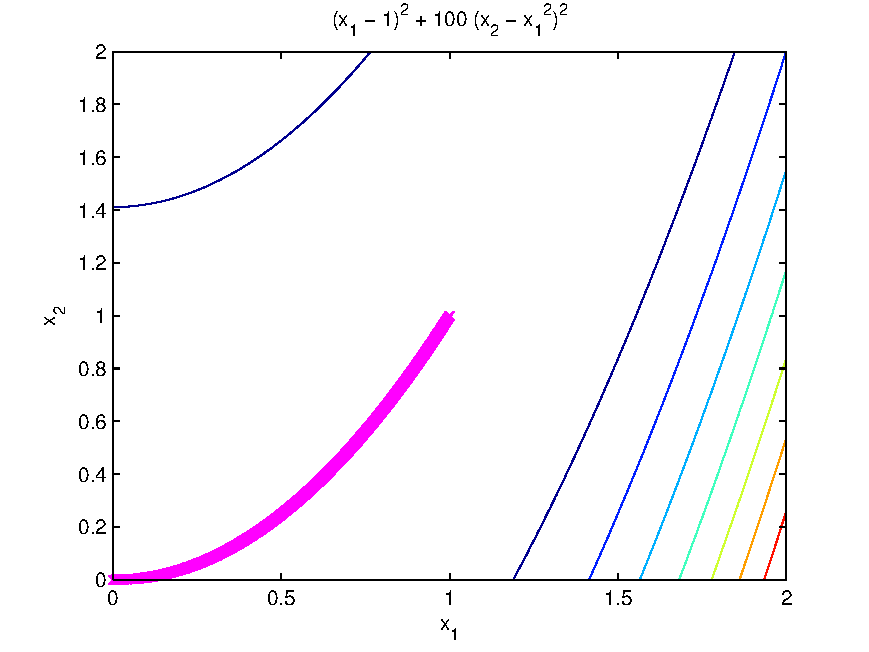
\includegraphics[width=4in, height=3in] {pic2.pdf}
	\caption{(a) contours and convergence of gradient descent to (1,1)}
      \end{minipage}
  \end{figure}
  \begin{figure}[h!]
      \begin{minipage}{0.5\linewidth}
        \centering
	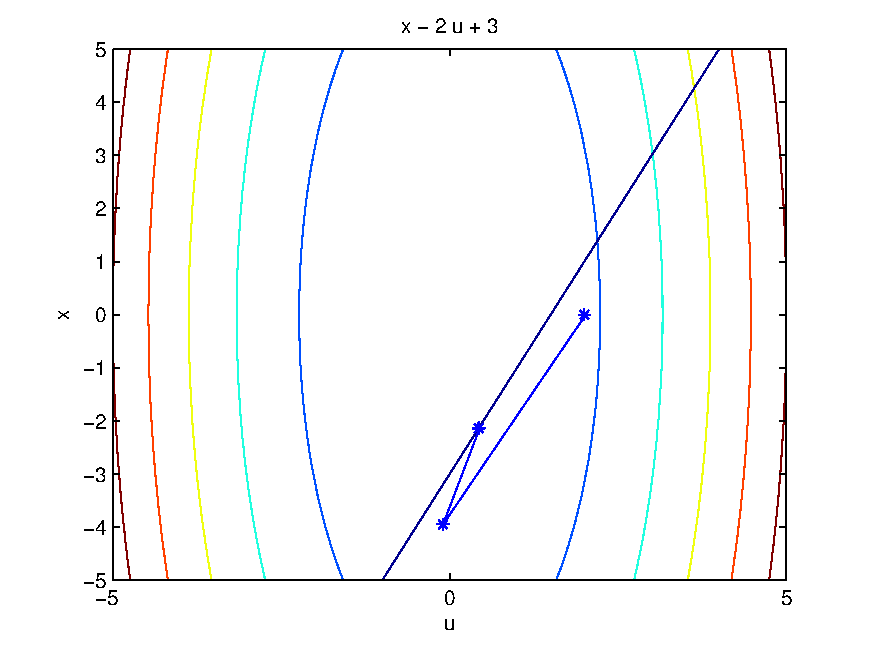
\includegraphics[width=4in, height = 3in] {pic3.pdf}
	\caption{(b) contour plot of constrained minimization for $L = x^2 + 10
u^2$}
      \end{minipage}
      \hspace{0.2in}
      \begin{minipage}{0.5\linewidth}
      \centering
	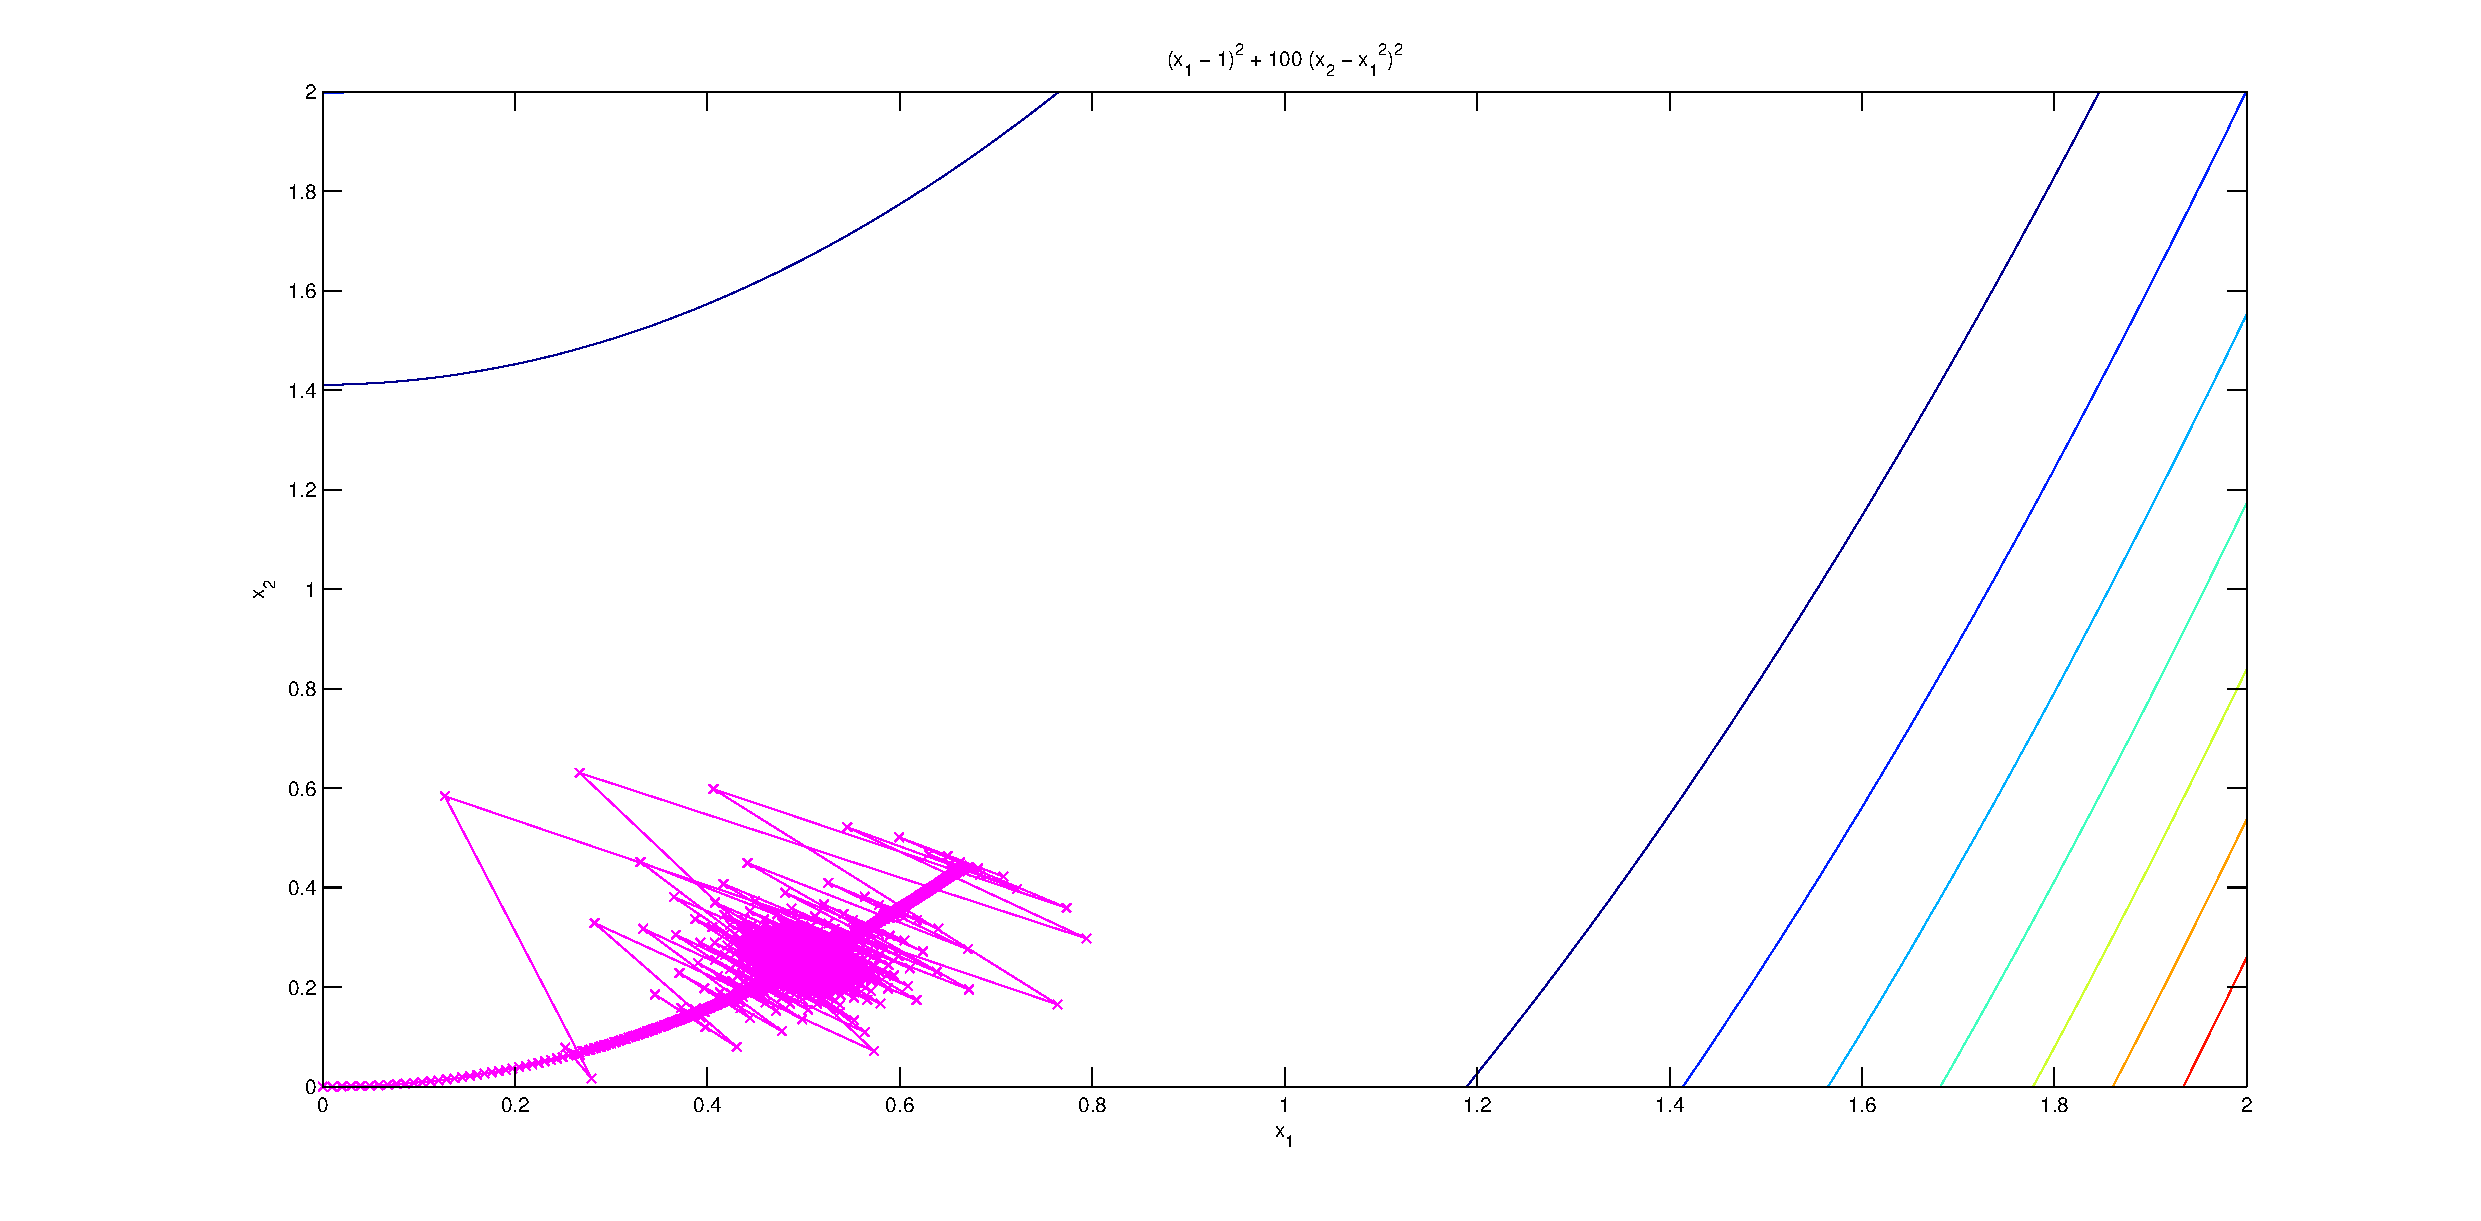
\includegraphics[width=4in, height = 3in] {pic5.pdf}
	\caption{(a) divergence for step size 0.005}
      \end{minipage}
  \end{figure}
  %%%%%%%%%%%%%%%Question 5%%%%%%%%%%%%%%%%%%%%%%%%
 \item Minimization problem stated as:
 \begin{align*}
  f^k(d) &= f(x^k) + \nabla f(x^k)^T d + \frac{1}{2} d^T \nabla^2 f(x^k) d \quad
d \in \mathbb{R}^n\\
  s.t \quad \|d\| &\leq \gamma ^{k}\\
 \end{align*}
 If the constraint is active it is treated as an equality and following Lagrange
multipliers method:
 \begin{align*}
  f(d) &= \|d\| -\gamma^k = \sqrt{d^T d} - \gamma^k \\
  L^\prime(d) &= f(x^k) + \nabla f(x^k)^T d + \frac{1}{2} d^T \nabla^2 f(x^k) d
+ \lambda(\sqrt{d^T d} - \gamma^k) \quad \lambda \geq 0\\
  \frac{\partial L^\prime}{\partial d} &= \nabla f(x^k)^T + d^T \nabla^2 f(x^k)
+ \lambda(\frac{1}{2 \sqrt{d^T d}}d^T) = 0\\
  \frac{\partial L^\prime}{\partial \lambda} &= \sqrt{d^T d} - \gamma^k = 0 \\ 
  \Rightarrow -\nabla f(x^k)^T&= d^T \left( \nabla^2 f(x^k) + \frac{\lambda}{
\gamma^k }I\right) \\
  \Rightarrow \left( \nabla^2 f(x^k) + \delta^k I\right)d &= -\nabla f(x^k)\quad
\text{Since hessian and Identity are both symmetric}\\
 \end{align*}
 Thus we have shown that the constrained optimization problem is equivalent to
solving the above form of matrix equations for $\delta^k$ and d. We need to choose the right $\delta^k$ so that the value of $d^Td < {\gamma^{k}}^2$. A reasonable choice of $\delta^k$ is
$max\{-eig(\nabla^2 f(x^k)),0\}+ \epsilon \quad \epsilon \geq 0 $. Since the eigen values of the incremented
Hessian is the sum of original eigenvalues and $\delta^k$. Such a choice will
ensure all the eigen values of $\left( \nabla^2 f(x^k) + \delta^k I\right)$ at least $\epsilon$. This satisfies the second order sufficiency condition for the Hessian.Also the value of 
$\epsilon$ should be found such that the value $\sqrt{d^Td} \leq \gamma^k$
% \begin{align*}
% \text{if } &\delta^k = max\{-eig(\nabla^2 f(x^k)),0\}+ \epsilon \quad \epsilon \geq 0 \\
%   &\Rightarrow d^T\left( \nabla^2 f(x^k) + \delta^k I\right)d = -d^T\nabla f(x^k) \geq d^T \mathit{\epsilon I}d = \epsilon {\gamma^k}^2\quad\\
%   &\Rightarrow 0 \leq \epsilon \leq \frac{-d^T \nabla f(x^k)}{{\gamma^k}^2}
% \end{align*}
% 
%%%%%%%%%%%%%%%%Problem 5%%%%%%%%%%%%%%
\item Paper: \textbf{Arthur Bryson Optimal Control 1950-1985}

This paper describes the efforts of various authors in a 35 year period in the field of optimal control.

\textbf{History of Calculus of Variations}

\emph{Roots from calculus of variations}\\
Optimal control can be regarded as an extension of calculus of variations. The paper describes some of the very early optimization problems posed by Galileo and Bernoulli(1600's) such as brachistochrone problem (shape of wire to minimize bead travel time); the drag nose shapes of projectile and other such problems. These were solved using Calculus of variations invented by Sir Newton and coinvented by Lebiniz. 
Based on these works Euler and Lagrange(1700's) have proposed the first order necessary conditions for a stationary solution namely Euler-Lagrange equations. 
The first-order conditions for generalizations from calculus of variations have been discovered in 1750-1850 by the efforts of Legendre, Jacobi and Hamilton culminating in the Hamilton-Jacobi equations which formed basis for dynamic programming later on.
The formal rigorous mathematical structure has finally been in place by efforts of Weirstras and many others. Also at the same time many people were able to recognize the use of Calculus of Variations for engineering design.

\emph{Roots from Classical control theory}\\
Optimal control in earlier days seen as a tool for adjusting the control system's performance to satisfactory and improve performance. This involved tuning the gains of the control systems and several crietia such as Nquist criterions etc have been proposed in the frequency domain.
In 1960 Kalman proposed a method for measuring the performance of the system and controlling the feedback to the system known as LQR (Linear Quadratic Regulator). 

\emph{Roots in Random Processes}\\
Started with Einstein and extended by Wiener, Newton, Gould, Kalman etc culminating in Linear Quadratic Estimator( LQE). The Linear Quadratic Estimator and Regulator combined to form the Linear Quadratic Gaussian (LQG) compensator.
Roots in Non-Linear Programming
Kuhn and Tucker proposed necesary conditions for the optimization of a system under inequality constraints. This led to the non-linear programming codes which solve optimal trajectories etc under various constraints. 

\emph{Effects of Technology on Optimal Control}\\
The Non-Linear Programming was extremely benifited by the invent of computers. It provided the computational power to handle hundreds and thousands of variables in a Non-Linear Programming problem.

\textbf{Important concepts developed in Optimal Control}:\\

\emph{Dynamic Programming:}\quad 
This was invented by Bellman based on the Hamilton-Jacobi equations. It computes a set of extremal paths and an optimal return function along with the feedback required for such paths. These methods are not useful without approximating the system into a Linear Quadratic problem.

\emph{Maximum Principle}: \quad
It is based on extending the Weirstrass's necessary condition to bounded control functions. It deals with find one extremum at a time and is different from Dynamic programming

\emph{Calulating NonLinear Optimal Trajectories}
First trajectories were proposed for rockets with limited fuel by Godard and were solved both analytically and numerically by various mathematicians. Later Gradient methods were proposed and coded by various people notably Hur and Bryson developed the MATLAB based gradient code. 
These problems have been applied to various real life situations in finding the right flight path to achieve a flight altitude in minimum time. Optimal control has also been used in finding optimal aerodynamic shapes etc.

\textbf{Handling of various special Cases in OC}

\emph{Inequality constraints:} \quad
Inequalities in control variables were handled by introducing slack variables or penality functions. State inequalities are harder to tackle and have been solved by Dreyfus and Speyer. 
\emph{Singular problems:} \quad
The cases where the second derivative goes to zero is known as a singular solution. Approximate solutions have been found and are in general difficult to find.
\emph{Inverse Optimal Control:} \quad
These were required to produce a control history for a required output history. The finding of feasible output histories is hard and involveds collocation methods and Non-Linear Programming concepts
\emph{Robust Optimal Control:} \quad
Linear Quadratic Gaussian controllers were not entirely robust to change in plant parameters. This came to light in using the controllers for space vehicles and new form of the problems known as $H_\infty$ has been proposed for robustness to unmodelled high frequency and is an ongoing research field.

Thus Optimal Control has a long history in various fields such as Calculus of Variations, Control Theory, Non-Linear Progamming and many other fields. It was applied to various real life problems during World War II  for finding optimal trajectories and also in designing various engineering structures. Many new areas where Optimal control needs to be applied are opening up showing a bright future for the field.


\end{enumerate} 
\begin{acknowledgements}
I hereby declare that I have not discussed this homework with anyone. The
solutions written here are my own work and  from lecture notes and sample code
provided by the professor. The paper summary contains lots of similarities with the original paper Arthur and Bryson ``Optimal Control - 1950-1985'', IEEE Control Systems, 1996

\flushright Gowtham Garimella
\end{acknowledgements}




\end{document}
